% !TEX program = xelatex
\usepackage{pgfpages}

\mode<presentation>
\title{Mid-term presentation}
\subtitle{\textit{Project Car Lane Detection using FPGAs}}
\author{Matthijs Bakker}

\usetheme{xilinx}

\begin{document}

	\frame{
		\titlepage

		\note[item]{Thank you for attending this presentation}
		\note[item]{Introducing the project and talking about the progress so far}

		\note[item]{Going off slides for 20 minutes}
		\note[item]{Last 5-10 minutes I will be showing the products with a live demonstration}
		\note[item]{Then, time for questions}
		\note[item]{Please fill in the feedback form that I have sent; I'd really appreciate the feedback because it helps me improve my presentation skills}
	}

	\frame{
		\frametitle{Did you know…}

		\note[item]{I would like to start off the presentation with a fact}
		\note[item]{Did you know that 45 percent of highway crashes in the United States only involve a single vehicle?}
		\begin{columns}
			\begin{column}{0.7\textwidth}
				… that 45\% of highway crashes  in the USA only involve a single vehicle?

		\bigskip

		\vspace{1em}
		\vspace{0.25cm}
		\vspace{2cm}

			\end{column}

			\begin{column}{0.3\textwidth}
				\begin{figure}
					\centering
					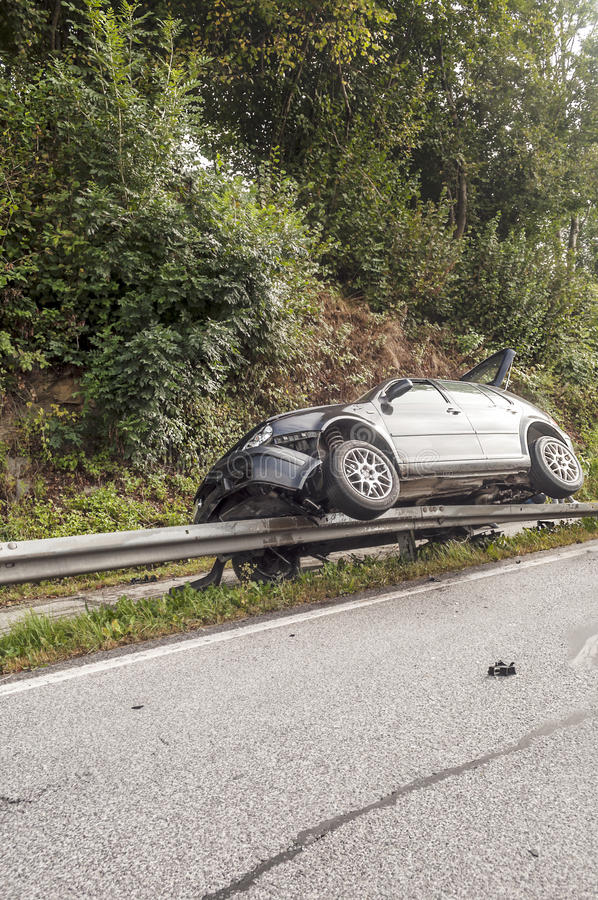
\includegraphics[width=\textwidth]{accident.jpg}
				\end{figure}
			\end{column}
		\end{columns}
		\let\thefootnote\relax\footnote{ad; C. Liu, et al., „Factors related to \dots~ run-off-road crashes”, \textit{NHTSA}, Nov. 2019.}
	}

	\frame{
		\frametitle{Did you know...}
		
		\note[item]{In 95 percent of these single vehicle crashes, the cause of the accident was attributed to the driver}

		\begin{columns}
			\begin{column}{0.7\textwidth}

		… that 45\% of highway crashes in the USA only involve a single vehicle?
		
		\bigskip

		… 95\% of these are attributed solely to the driver
		\vspace{0.25cm}
		\vspace{2cm}
			
			\end{column}

			\begin{column}{0.3\textwidth}
				\begin{figure}
					\centering
					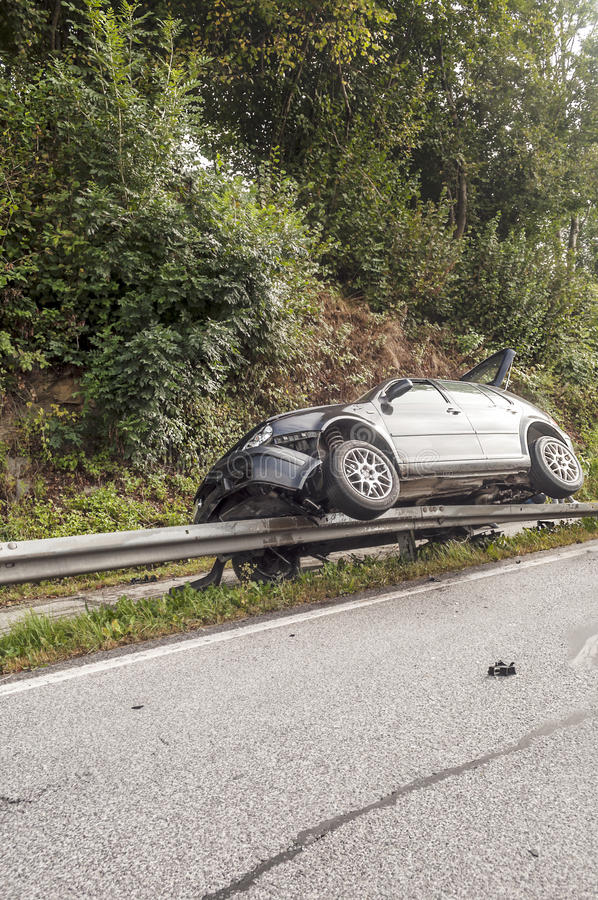
\includegraphics[width=\textwidth]{accident.jpg}
				\end{figure}
			\end{column}
		\end{columns}
		\let\thefootnote\relax\footnote{ad; C. Liu, et al., „Factors related to \dots~ run-off-road crashes”, \textit{NHTSA}, Nov. 2019.}
	}

	\frame{
		\frametitle{Did you know...}

		\textcolor{gray}{… that 45\% of highway crashes in the USA only involve a single vehicle?}
		
		\bigskip

		\textcolor{gray}{… 95\% of these are attributed solely to the driver}

		\bigskip

		Common causes are driver incapacitance:
		\vspace{0.25cm}

		\begin{itemize}

			\item Sleep deprivation
			\item Under the influence of alcohol

		\end{itemize}
		\let\thefootnote\relax\footnote{ad; C. Liu, et al., „Factors related to \dots~ run-off-road crashes”, \textit{NHTSA}, Nov. 2019.}
		\note[item]{The most common causes of these accidents are some kind of driver incapacitance, like}
		\note[item]{Sleep deprivation}
		\note[item]{Influence of alcohol or other substances}
		\note[item]{But, Not only are physical factors to blame: mental factors like distraction are also common}
		\note[item]{We have so many distractions around us nowadays; our phones are a good example of this}
		\note[item]{Red light? Let me just check my Twitter feed quickly}
	}

%	\frame{
%		\frametitle{What I will be talking about}
%		\framesubtitle{My really long subtitle goes here...}
%
%		\begin{itemize}
%
%			\item The premise of this project
%			\item What's the planning like?
%			\item My progress so far
%			\item What's to do in the future?
%
%		\end{itemize}
%	}

	\frame{
		\frametitle{The premise of this project}
	
		\note[item]{Combat driver incapacitance by making the car smarter and more autonomous}
		\note[item]{AROBS has an Advanced Driver Assistance System that is constantly being developed to make cars more autonomous}
		\note[item]{Next advancement towards the goal of fully autonomous driving is to make cars aware of the lane they are driving in}
		\note[item]{Warning systems can react when departing the lane; stick shaker, brakes}
		\note[item]{Project only revolves around detecting lane, not decisions made upon result}
		\note[item]{If we want mass adaptation, we need the solution to be low cost and low power}

		\begin{itemize}

			\item Autonomous driving
			\item Integration with existing ADAS
			\item Goal: detect car position within lane
			\item Low-cost universal solution

		\end{itemize}

		\vspace{0.5cm}
		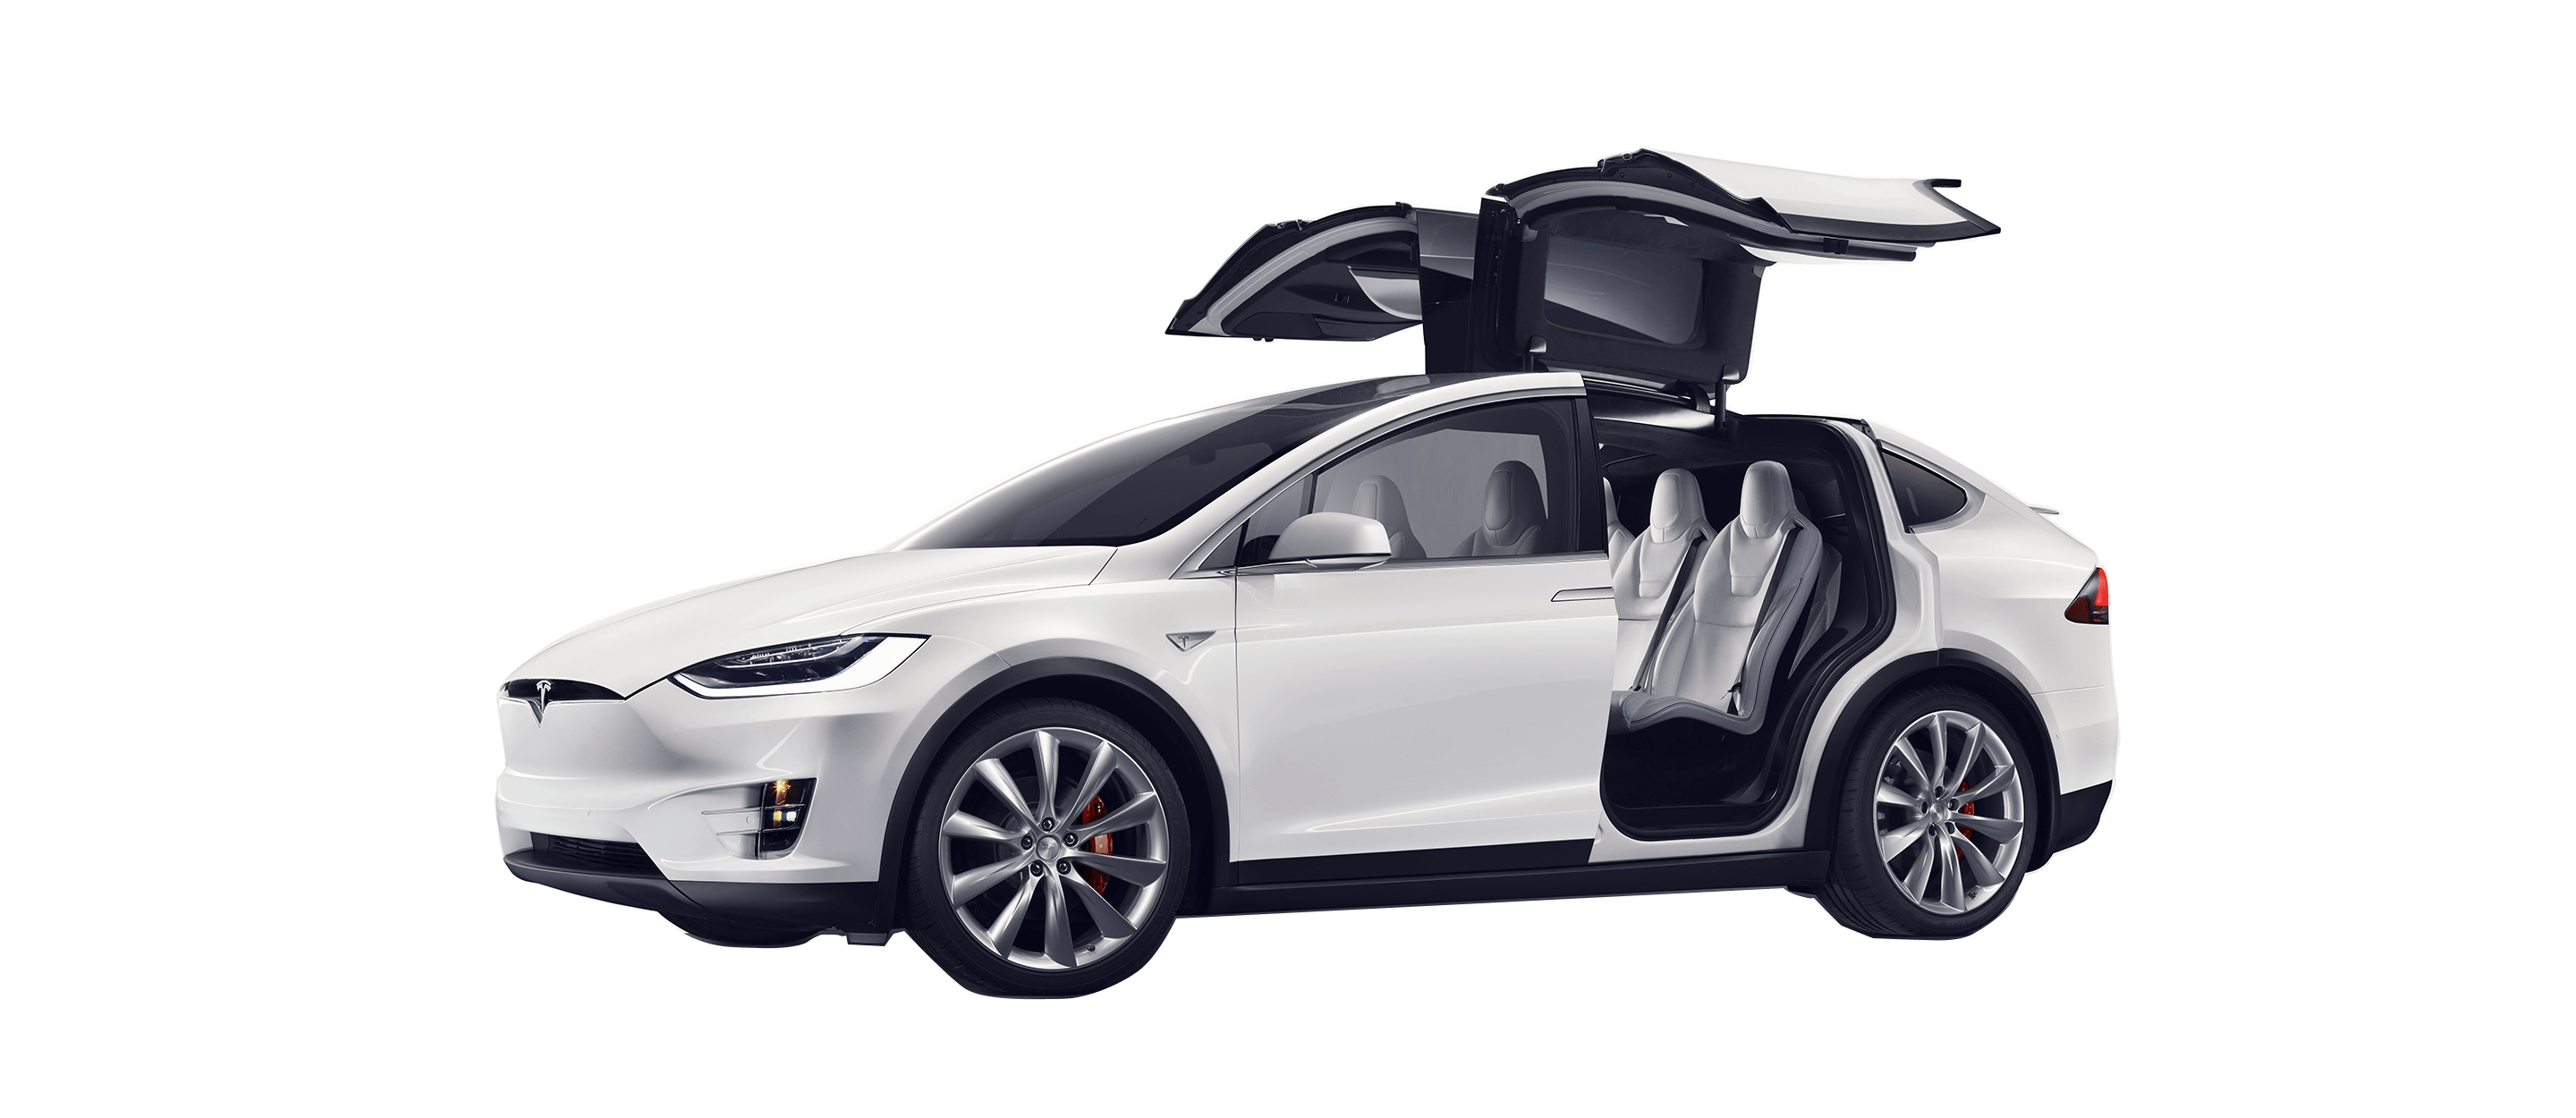
\includegraphics[width=0.45\textwidth]{tesla-model-x.png}
		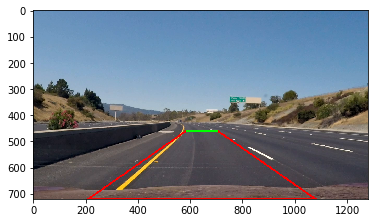
\includegraphics[width=0.5\textwidth]{goal.png}
	}

	\frame{
		\frametitle{How do we detect the lane markings?}
		\framesubtitle{My venture into computer vision}

		\note[item]{Now comes the important question: how do we detect the lane markings?}
		\note[item]{I chose a computer vision approach because it can be used without changes to the road surface; no special sensors or whatever; it can be integrated into the existing road network}
		\note[item]{A popular approach of detecting image lines within the computer vision field is by using the Hough transform; this is complex non-supervised algo}
		\note[item]{Before applying the Hough transform we need to pre-process the video feed because the Hough transform is easily influenced by noise and artifacts in the image}
		\note[item]{We do this by applying specific image filters}
		\note[item]{I spent five weeks on creating a test program -- handmade}

		\vspace{0.75cm}

		\begin{itemize}

			\item Camera mounted on dashboard
			\item Preprocessing the image to highlight lane markings
			\item Line detection using Hough Transform
			\item Minimize amount of false positives

		\end{itemize}

		\vspace{0.25cm}

		\setbeamertemplate{caption}{\raggedright\insertcaption\par\small}
		\begin{columns}[onlytextwidth]
			\begin{column}{.32\textwidth}
				\begin{figure}
					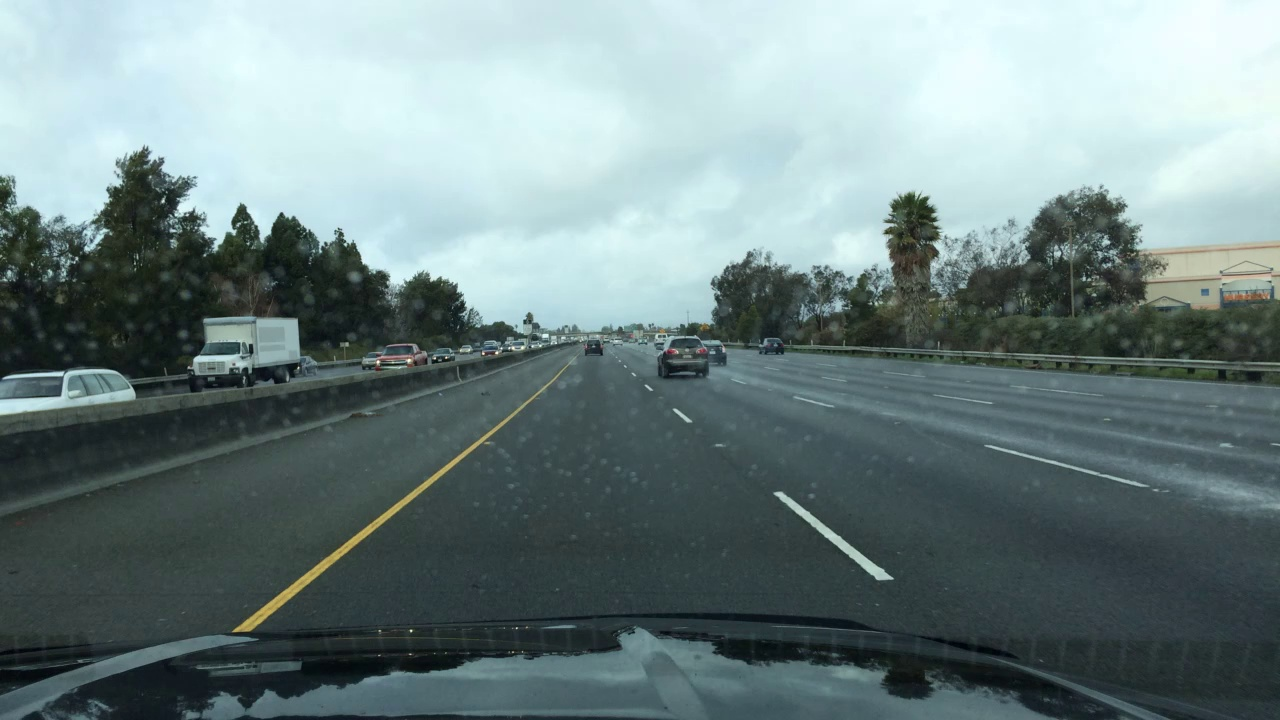
\includegraphics[width=\textwidth]{3b0cba4e-59a949a7.jpg}
					\caption{Original image}
				\end{figure}
			\end{column}
			\hfill
			\begin{column}{.32\textwidth}
				\begin{figure}
					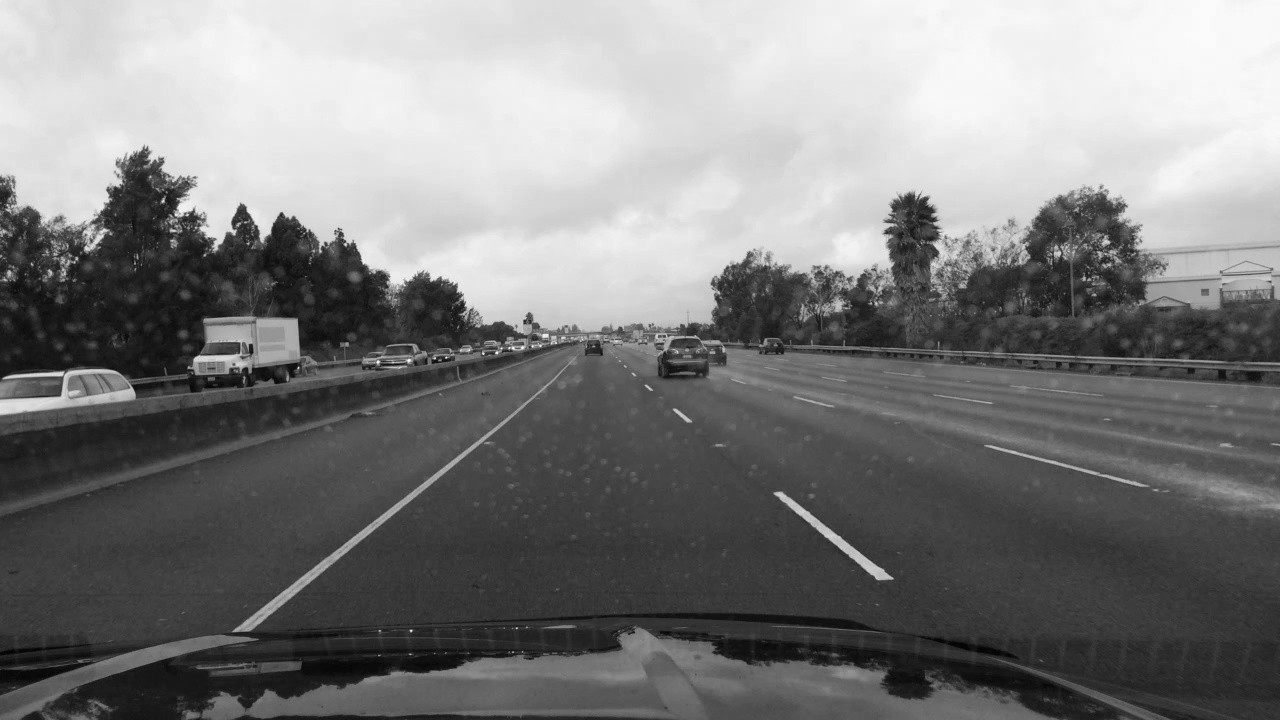
\includegraphics[width=\textwidth]{3b0cba4e-59a949a7.grayscale.out.jpg}
					\caption{After grayscale filter}
				\end{figure}
			\end{column}
			\hfill
			\begin{column}{.32\textwidth}
				\begin{figure}
					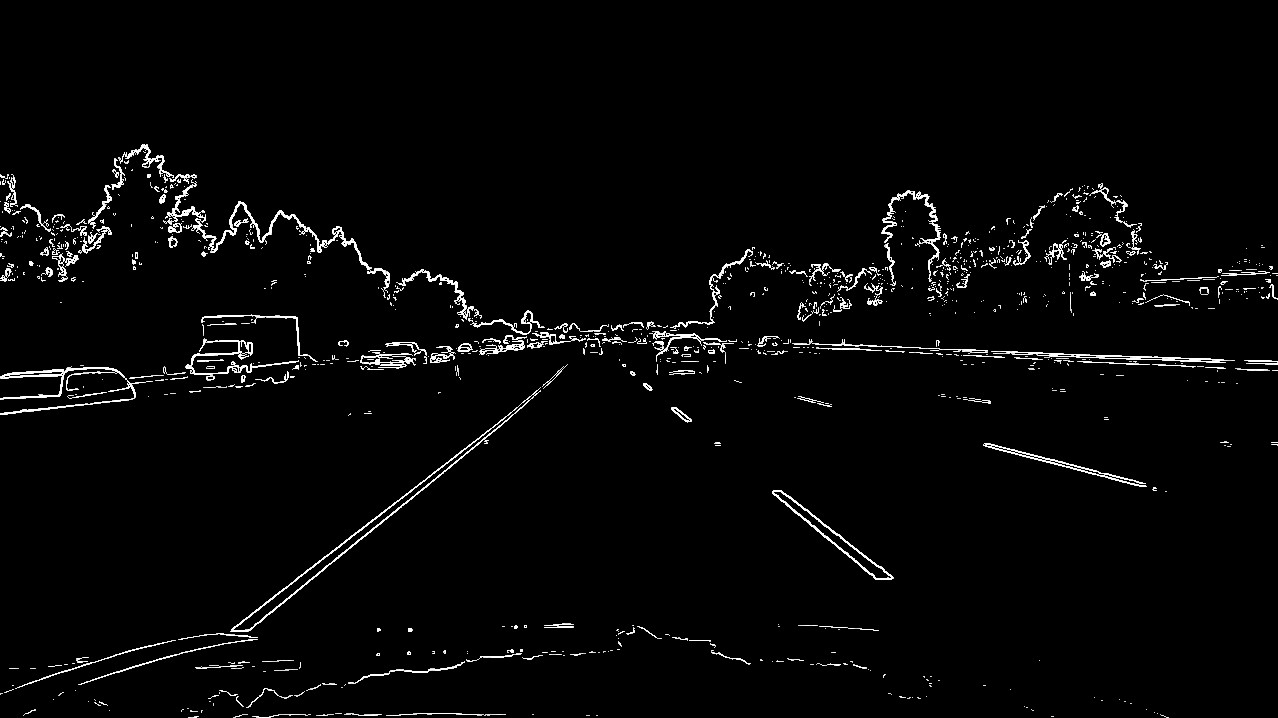
\includegraphics[width=\textwidth]{3b0cba4e-59a949a7.grayscale.out.sobel.out.jpg}
					\caption{After Sobel filter}
				\end{figure}
			\end{column}
		\end{columns}
	}

	\frame{
		\frametitle{What is an FPGA?}

		\begin{itemize}
			\note[item]{An FPGA is a bunch of wires and logic gates that are not connected by default}
			\note[item]{Out of the box, an FPGA does not do anything}
			\note[item]{The developer has to arrange the wires and logic gates for it to function in a particular way}
			\note[item]{The beauty of FPGAs = they are reconfigurable HW = you can make them do anything = any combination of wires and logic is possible = hardware is endless}
			\note[item]{Whereas microcontrollers and processors are predefined hardware. They have a specific function that cannot be changed, you cannot make it do any other thing than it is designed for}
			\note[item]{We can design the hardware (arrangement of wires and logic gates) in the FPGA to do any function, like take video input and process the video}
			\note[item]{A microcontroller can only process 1 pixel per clock pulse at max, whereas an FPGA can process however many pixels per clock pulse as the design can handle}
			\item High throughput parallel processing

			\note[item]{Another big player in the video processing field: the GPU}
			\note[item]{Why use an FPGA over a GPU?}
			\note[item]{Cost: Popular GPU-accelerated (Nvidia Jetson) = expensive}
			\note[item]{Make into an ASIC}
			\note[item]{Two major players: Intel and AMD}
			\item GPU prices are rising
			\item Xilinx acquired by AMD last February\footnote{J. L. Lee, „AMD closes record \dots~ purchase of Xilinx”, \textit{Reuters}, Feb. 2022.}

		\end{itemize}

		\vspace{0.6cm}
		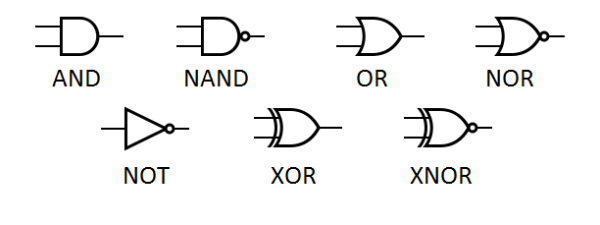
\includegraphics[width=0.5\textwidth]{gates.png}
		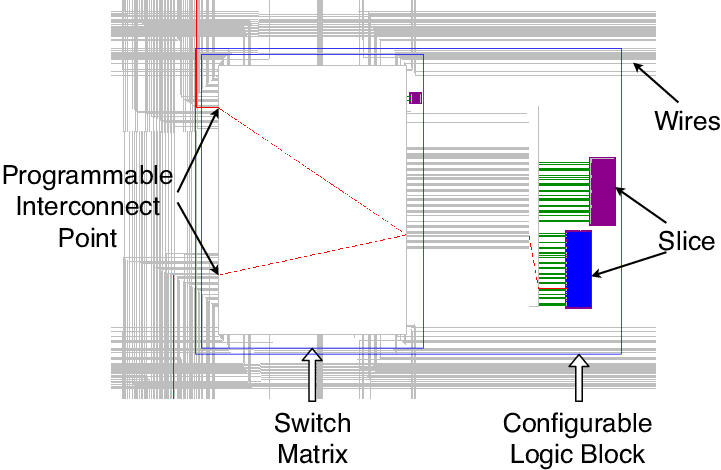
\includegraphics[width=0.45\textwidth]{fpga.png}
	}

	\frame {
		\frametitle{How will I implement the system on an FPGA?}
		\framesubtitle{}

		\note[item]{Over the next 7 weeks I will implement the processing pipeline}
		\note[item]{Already started: MWE in demo at the end}
		\note[item]{Creating hardware logic is very time consuming, therefore I will use HLS}
		\note[item]{HLS is a way of describing the hardware, as you would do in a hardware description language, but at a higher level}
		\note[item]{Think of it as C vs Assembly language; you can do the same thing, but C is 20x more efficient}

		\begin{itemize}

			\item High Level Synthesis
			\item CPU for offloading images and results

		\end{itemize}

		\vspace{0.4cm}
		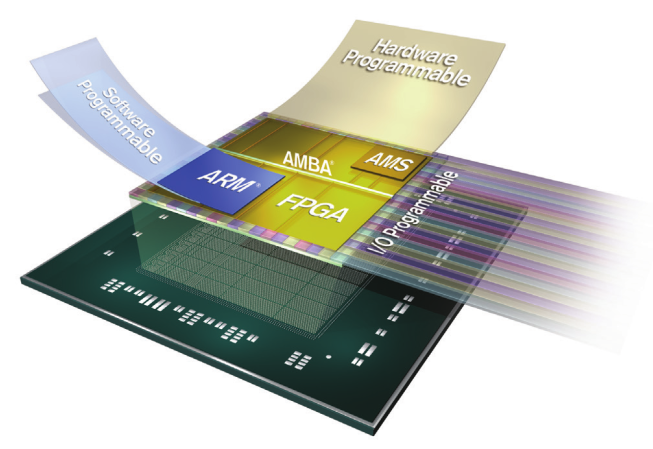
\includegraphics[width=0.5\textwidth]{soc.png}
		\hspace{0.2cm}
		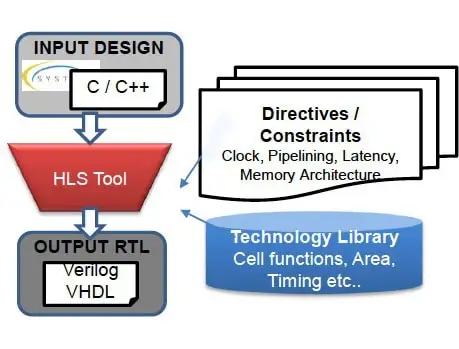
\includegraphics[width=0.45\textwidth]{hls.png}
	}

	\frame{
		\frametitle{Finishing up…}

		\begin{itemize}

			\item Live demonstration
			\item Time for questions
			\item Feedback form

		\end{itemize}

		\note[item]{Switch over to laptop for demo!}
	}

\end{document}
